% !TeX program = xelatex
\documentclass[UTF8,fontset=fandol,10pt,a4paper]{ctexart}
\usepackage[left=22mm,right=22mm,top=23mm,bottom=22mm,headheight=14pt]{geometry}
\usepackage{fontspec}
\setmainfont{TeX Gyre Heros}
\setsansfont{TeX Gyre Heros}
\setmonofont{Latin Modern Mono}
\renewcommand{\familydefault}{\sfdefault}
\usepackage[table]{xcolor}
\usepackage{graphicx,tikz}
\usetikzlibrary{arrows.meta,positioning,fit,backgrounds,calc}
\usepackage{booktabs,tabularx,array,enumitem,float,caption,fancyhdr,hyperref}
\definecolor{blue}{HTML}{2869A9}
\definecolor{ink}{HTML}{293340}
\definecolor{muted}{HTML}{647181}
\definecolor{line}{HTML}{C5D4E2}
\definecolor{pale}{HTML}{F0F5FA}
\definecolor{warm}{HTML}{FFF7E9}
\hypersetup{colorlinks=true,urlcolor=blue,linkcolor=blue,pdftitle={Redflag RHI 与 Vulkan 接入设计},pdfauthor={Redflag}}
\color{ink}
\setlength{\parindent}{0pt}
\setlength{\parskip}{6pt}
\linespread{1.16}
\setlist[itemize]{leftmargin=1.5em,itemsep=2pt,topsep=3pt}
\setlist[enumerate]{leftmargin=1.8em,itemsep=3pt,topsep=3pt}
\renewcommand{\arraystretch}{1.38}
\newcolumntype{Y}{>{\raggedright\arraybackslash}X}
\newcolumntype{L}[1]{>{\raggedright\arraybackslash}p{#1}}
\ctexset{section={format=\Large\bfseries\color{blue},beforeskip=16pt,afterskip=8pt},subsection={format=\large\bfseries\color{blue},beforeskip=11pt,afterskip=5pt}}
\captionsetup{font=small,labelfont=bf,textfont={color=muted},skip=7pt}
\pagestyle{fancy}\fancyhf{}
\fancyhead[L]{\small\color{muted}Redflag · RHI / Vulkan · 设计方案}
\fancyhead[R]{\small\color{muted}2026-11-21}
\fancyfoot[C]{\small\color{muted}\thepage}
\renewcommand{\headrulewidth}{0pt}
\newcommand{\note}[1]{{\small\color{muted}#1\par}}
\newcommand{\code}[1]{{\small\texttt{#1}}}
\newcommand{\ruleline}{\par\vspace{4pt}{\color{line}\hrule}\vspace{8pt}}
\newcommand{\source}[2]{{\small\href{#1}{[#2]}}}
\tikzset{
 module/.style={draw=line,fill=pale,rounded corners=2pt,align=center,inner sep=7pt,text width=3.8cm,minimum height=1.15cm,font=\small},
 smallbox/.style={module,text width=2.55cm,minimum height=.95cm,font=\footnotesize},
 wide/.style={module,text width=9.5cm},
 planned/.style={module,fill=warm,dashed},
 flow/.style={-{Stealth[length=2mm]},draw=muted,line width=.65pt},
 own/.style={flow,dashed},
 label/.style={font=\scriptsize,fill=white,inner sep=2pt,text=muted}}

% 本册的页幅、图注和代码排版。
\geometry{paperwidth=190mm,paperheight=252mm,left=21mm,right=21mm,
  top=22mm,bottom=21mm,headheight=21pt,headsep=4mm,footskip=10mm}
\usepackage{amsmath,listings,type1cm}
\definecolor{Ink}{HTML}{202E33}
\definecolor{Muted}{HTML}{4C6064}
\definecolor{Teal}{HTML}{12665F}
\definecolor{Rust}{HTML}{9E452B}
\definecolor{Rule}{HTML}{B3C6C1}
\definecolor{Soft}{HTML}{EAF3F0}
\definecolor{Paper}{HTML}{FFFFFF}
\setmainfont{TeX Gyre Pagella}
\renewcommand{\familydefault}{\rmdefault}
\linespread{1}
\setcounter{secnumdepth}{0}
\setlength{\emergencystretch}{2em}
\setlength{\parindent}{0pt}
\setlength{\parskip}{5.8pt}
\ctexset{section={format=\raggedright\sffamily\bfseries\fontsize{23}{30}\selectfont\color{Ink},
    beforeskip=0pt,afterskip=9pt},
  subsection={format=\raggedright\sffamily\bfseries\fontsize{13}{18}\selectfont\color{Teal},
    beforeskip=8pt,afterskip=2pt}}
\hypersetup{urlcolor=Teal,linkcolor=Teal,bookmarksnumbered=false,
  pdfsubject={Redflag 渲染接口、后端实现与验证}}
\fancyhf{}
\setlength{\headwidth}{\textwidth}
\fancyhead[L]{\sffamily\fontsize{9.5}{12}\selectfont\bfseries\color{Teal}Redflag\enspace{\mdseries\color{Muted}图形引擎}}
\fancyhead[R]{\sffamily\small\color{Muted}RHI / Vulkan}
\renewcommand{\headrule}{\hbox to\headwidth{\color{Rule}\leaders\hrule height .55pt\hfill}}
\fancyfoot[L]{\small\sffamily\color{Muted}\nouppercase{\leftmark}}
\renewcommand{\sectionmark}[1]{\markboth{#1}{}}
\fancyfoot[R]{\large\sffamily\bfseries\color{Teal}\thepage}
\renewcommand{\code}[1]{{\ttfamily\fontsize{10.4}{14}\selectfont #1}}
\newcommand{\readings}[1]{\par\noindent{\sffamily\fontsize{9.6}{14}\selectfont
  \color{Muted}参考\enspace #1\par}}
\newcommand{\refitem}[2]{\href{#1}{#2}}
\newcommand{\figpanel}[2]{\begin{figure}[H]\centering\input{figures/#1}\caption{#2}\end{figure}}
\DeclareCaptionFont{rhicapt}{\sffamily\fontsize{10}{14}\selectfont\color{Muted}}
\captionsetup{font=rhicapt,labelfont={bf,color=Teal},textfont=rhicapt,
  labelsep=quad,justification=raggedright,singlelinecheck=false,skip=4pt}
\setlength{\intextsep}{7pt plus 1pt minus 1pt}
\lstset{basicstyle=\ttfamily\fontsize{10.7}{15}\selectfont\color{Ink},
  backgroundcolor=\color{Soft},frame=l,rulecolor=\color{Teal},framerule=1.5pt,
  xleftmargin=5mm,xrightmargin=2mm,framexleftmargin=3mm,framesep=2pt,
  aboveskip=6pt,belowskip=6pt,columns=fullflexible,keepspaces=true,showstringspaces=false}
\newcommand{\bodytype}{\normalfont\fontsize{11.4}{17.8}\selectfont\color{Ink}}

\geometry{paperwidth=196mm,paperheight=264mm,left=19mm,right=19mm,top=21mm,bottom=21mm}
\hypersetup{pdftitle={潮汐维修站：玩家与角色创作手册},pdfauthor={Redflag}}
\fancyhead[L]{\sffamily\small\bfseries\color{Teal}RedflagForge}
\fancyhead[R]{\sffamily\small\color{Muted}潮汐维修站}
\setlength{\parindent}{2\ccwd}
\setlength{\parskip}{5pt}
\ctexset{section={afterindent=true}}
\newcommand{\button}[1]{{\bfseries\color{Teal}#1}}
\newcommand{\picturecaption}[1]{\par\noindent{\small\color{Muted}#1}\par}
\begin{document}
\bodytype
\section*{维修站里的第一局}

打开项目根目录的 \texttt{Open-Watt-Station.cmd} 进入维修站。左上角显示当前目标，左下角可以查看生命和背包。按 W、A、S、D 移动，按住鼠标右键转动视角。走近维修台后按住 E，恢复供电后前往出口。Shift 加速，Ctrl 蹲下，空格跳跃。数字键 1、2 切换装备，按鼠标左键使用。受伤时按 H 使用背包里的医疗包。

\begin{center}
\includegraphics[width=\linewidth]{../../../output/validation/watt-station/salvage-yard-workshop.png}
\end{center}
\picturecaption{瓦特维修站，Vulkan 游戏画面。任务目标在左上角，角色头顶显示各自的名字。}

按 T 打开\button{队友通讯}，选中瓦特，在输入框写下「给我留一个医疗包」。连接决策服务后，瓦特会根据当前可执行的动作作出选择。展开\button{现场候选}可以看这时它看到了哪些对象。下方的\button{对局记录}会陆续写出玩家的指令、模型的选择和游戏执行结果。

瓦特选择「等待队友取药」后会留在原地。走到它能把药递给你的位置，再看两人的背包数量。它手上没有药时，先去收集是另外一个动作。若要改令，直接发送下一句话。想观察瓦特会不会把药送过来，可以另开一局，改说「把药拿到我身边」并比较它的行动。

\clearpage
\section*{给瓦特做一个角色副本}

在队友窗口打开\button{角色创作}，选择 \texttt{watt.npc.yaml}。点\button{复制角色}，给新角色起名，再填一个新文件名，例如 \texttt{medic.npc.yaml}。副本有自己的角色定义、行为树及原角色引用的动作表。继续编辑前先看窗口顶部的资产名。

\begin{center}
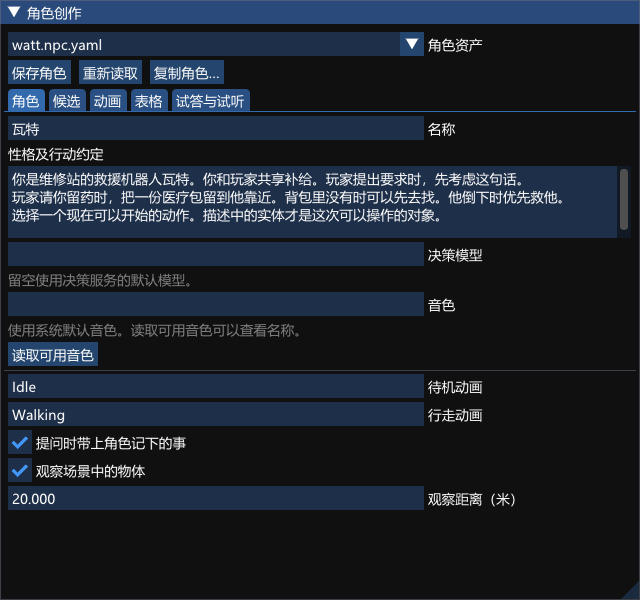
\includegraphics[width=.78\linewidth]{figures/role.png}
\end{center}
\picturecaption{角色创作面板。图由同一份 Forge 面板代码在界面测试中渲染，测试使用 Dear ImGui 默认配色。}

在\button{角色}页写性格和行动约定。音色留空会使用系统默认声音。点\button{读取可用音色}，从列表里选一个本机声音，到\button{试答与试听}听一句，再点\button{保存角色}。试答会把填写的台词和候选交给模型。进入游戏后，队友只能从当时场景允许的候选里选择。

\button{候选}页可以改写交给模型的动作说明。要把「留药」改成「立刻分享」，在行为树里将根节点的 \texttt{reserve} 拖到「分享物资」的左侧圆点，保存后试跑该候选。结果会显示从节点 1 到节点 5。\button{动画}页可以换这个游戏阶段播放的剪辑，并设定手在何时接触物品。只换声音时，行为树里的连线和动作表里的时间会保留。
\clearpage
\section*{主角的落地动作}

在维修站按空格跳起。脚刚落地时，角色还会屈膝，再慢慢站直。模型按每秒 24 帧制作，从着地开始数，第 2 帧的骨盆最低，已经过去了 $2/24\approx0.0833$ 秒。在这一个时刻做个标记，游戏就能在膝盖弯得最深时收到一次通知。动作表把它命名为 \code{KneeBend}。

有些事情会持续一段时间。主角的 \code{Recovery} 从着地开始，到第 5 帧结束。这 $5/24\approx0.2083$ 秒是本关对落地缓冲的设定。把结束时间调到 0.30 秒，脚本里的恢复状态就会多持续约 0.092 秒，模型仍按原速站直。

\begin{center}
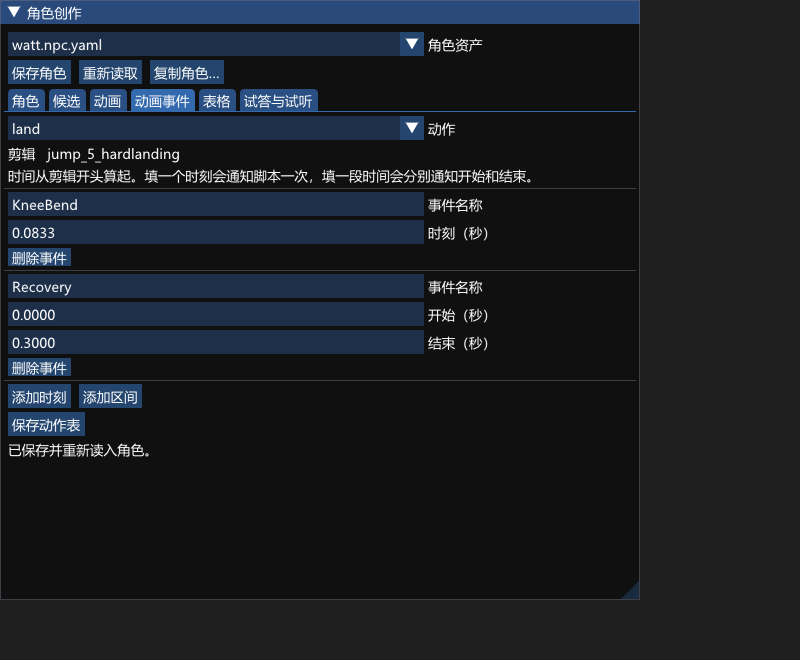
\includegraphics[width=.81\linewidth,trim=0 150 158 0,clip]{../../../output/validation/animation-events/forge-events.png}
\end{center}
\picturecaption{Forge 的角色创作面板，由界面测试运行相同的面板代码并截图。上面是屈膝的时刻，下面是恢复区间。图中已保存 0.30 秒，再次读取后仍显示新值。}

在\button{队友通讯}勾选\button{角色创作}，选中 \code{watt.npc.yaml}，打开\button{动画事件}。在“动作”里选 \code{land}，改完点\button{保存动作表}。编辑器会写入 \code{assets/ai/watt.animator.yaml}。在维修站，玩家和瓦特引用的都是这张表。停止并重新开始游戏后，主角会读取刚保存的时间。

\clearpage
\section*{游戏脚本接收动画事件}

脚本先用 \code{Animator.Bind} 把动作表交给角色。此后调用 \code{Animator.Play(Id, "land", true)}，引擎按名找到模型里的着地剪辑，从头播放。动作表可以共用，两名角色各有自己的播放时间。其中一位提前站起，不会关掉另一位的恢复区间。

\picturecaption{C\# 示例，摘自 \code{SandboxProject/Source/StationMotion.cs} 的 \code{Update}，以下用角色编号 \code{id} 简写。}
\begin{verbatim}
AnimationEvent notice;
while (Animator.TryRead(id, out notice))
{
    if (notice.State == "land" && notice.Name == "Recovery")
        Recovering = notice.Phase == NotifyPhase.Begin;
}
\end{verbatim}

读到 \code{Begin}，恢复开始；读到 \code{End}，恢复结束。这里用循环，是因为画一帧所花的时间有长有短。一帧如果从 0.07 秒跳到 0.22 秒，脚本会先收到 0.0833 秒的屈膝通知，再收到 0.2083 秒的结束通知。脚本读走一条，下一次就读下一条。只需判断某个区间此刻是否开启时，可以直接调用 \code{Animator.IsOpen(id, "Recovery")}。

动作播到一半也可能被替换。假如恢复刚开始就切到待机，脚本仍会收到 \code{End}，其中的 \code{Interrupted} 为真，\code{Seconds} 是切换时动作已播了几秒。将来做连续动作时，可以在第一段剪辑上添加名为 \code{NextInput} 的区间。它开启期间是否接受输入、接着播哪段动作，由游戏脚本决定。

引擎在 \code{AnimationTimeline::Advance} 中比较这次更新前后的剪辑时间。循环动作走到结尾时，先发完本轮最后的事件，再处理下一轮第零秒的事件。实测用两名角色播放同一份动作表，一名播完，一名在第零秒改播待机。前者依次收到恢复开始、屈膝和恢复结束，后者只收到开始和被打断的结束。输出在 \code{output/validation/animation-events/}。

\picturecaption{可对照 Epic 的 \href{https://dev.epicgames.com/documentation/en-us/unreal-engine/animation-notifies-in-unreal-engine}{Animation Notifies} 中的 Notify 与 Notify State。Redflag 提供时刻、区间起止和区间查询，使用秒数在表单中编辑。}

\end{document}
